% -*- coding: utf-8 -*-
\newpage
\section{Creation of a Geodesic Polyhedron (Icosphere)}\label{icosphereGeo}

To initialise the gradient path tracing process, we need to generate a structure
that resembles a sphere around the (R/C)CP. Computationally, this involves
implementing a set of equidistant points around the CP, which will serve as
starting points for tracing the gradient.

A geodesic polyhedron provides an effective means of distributing equidistant
points. It offers a balance between computational efficiency and accuracy.
This can be achieved in two main ways: the brute-force method and the recursive
method.

While the recursive method is more elegant and efficient for constructing
higher-order geodesic polyhedra, the brute-force method is better suited to our
requirements. The polyhedra we use do not demand a high level of recursion, and
as illustrated in Figure \ref{ico_time}, for the levels of icosphere relevant
to our study, the brute-force method is computationally less expensive.

\begin{figure}[h]
  \centering
  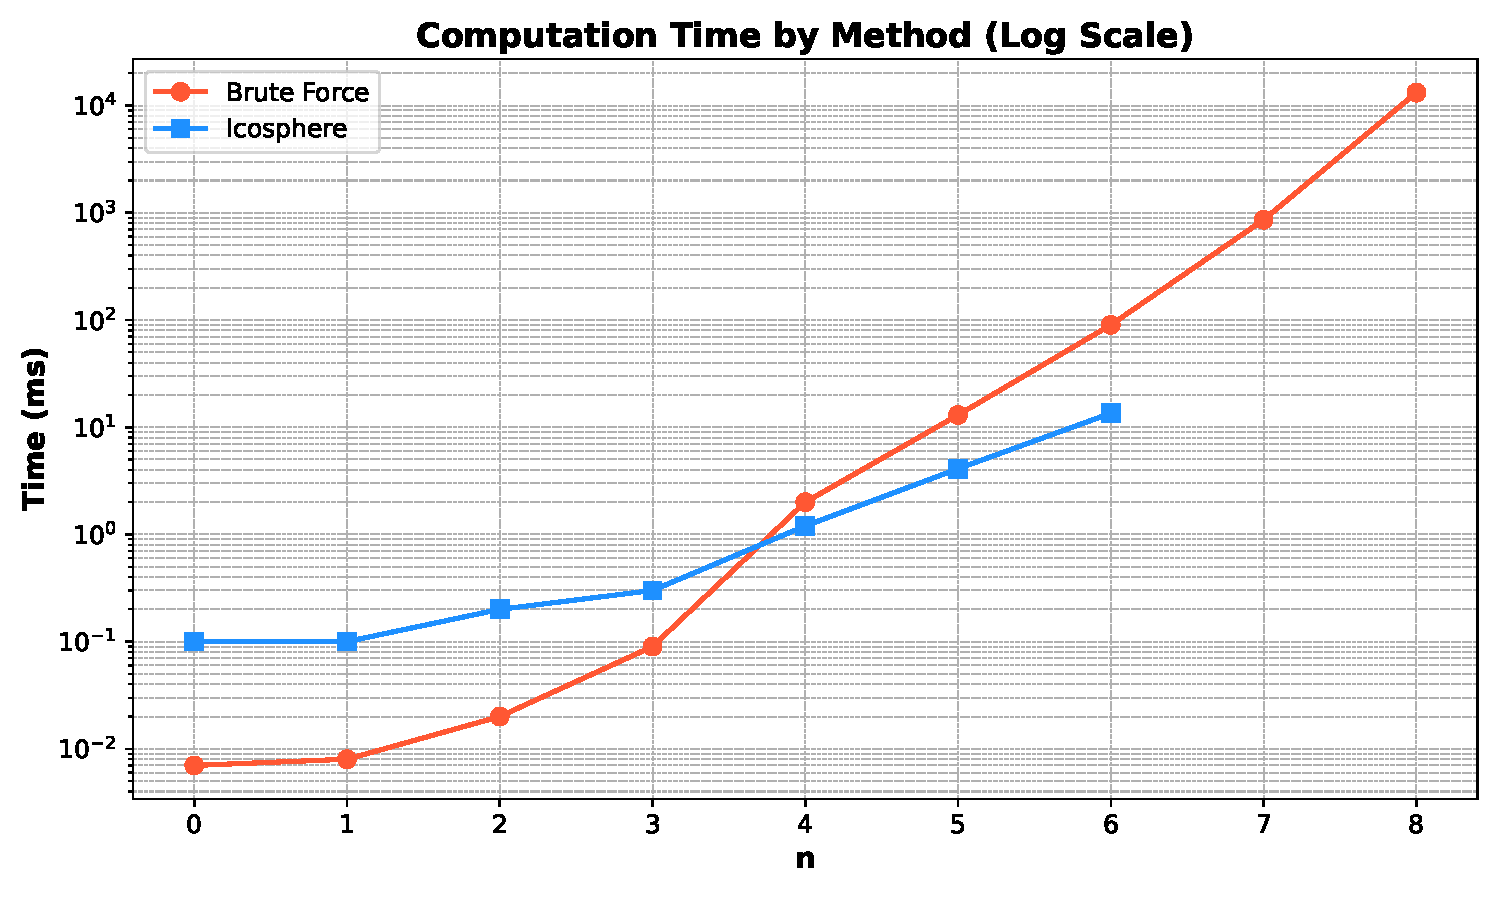
\includegraphics[width=0.8\textwidth]{img/computation_time.pdf}
  \caption{Time comparison between the brute-force and recursive methods for creating
  an icosphere, time in milliseconds.}
  \label{ico_time}
\end{figure}

The brute-force method is detailed in Algorithm \ref{brutef_algo}, while the
recursive method is described in Algorithm \ref{recursive_algo}. 

\newpage
\vspace*{4cm}

\begin{algorithm}[h]

  $\varphi \leftarrow \frac{1 + \sqrt{5}}{2}$\;
  radius $\leftarrow$ $\sqrt{2 + \varphi}$\;
  norm $\leftarrow$ $2\varphi$\;
  nver $\leftarrow$ $10 \cdot 4^{order} + 2$ \tcp*{number of vertices}
  edge $\leftarrow$ 2 \tcp*{analytical edge length}
  vertex $\leftarrow$ \texttt{zeros((nver, 3))}\;
  vertex[1:12,:] $\leftarrow$ [0, $\pm1$, $\pm\varphi$], [$\pm1$, $\pm\varphi$, 0], [$\pm\varphi$, 0, $\pm1$]

  \For{i $\gets 1$ \KwTo order}{
    nverb $\leftarrow$ $10 \times 4^{i-1} + 2$ \tcp*{number of vertices at previous order}
    l $\leftarrow$ nverb\;
    \For{j $\gets 1$ \KwTo nverb-1}{
      \For{k $\gets j+1$ \KwTo nverb}{
        \uIf{\texttt{distance(j,k)} $\leq$ edge}{
          l $\gets$ l + 1\;
          vertex[l,:] $\leftarrow$ radius $\times$ \texttt{midPoint(j,k)}/norm\;
        }
      }
    }
    edge $\leftarrow$ \texttt{distance(vertex[1,:], vertex[nverb+1,:])}
  }

  \caption{Brute-force method for creating an icosphere.}
  \label{brutef_algo}
\end{algorithm}

\vfill%
\newpage
\vspace*{1cm}

\begin{algorithm}[h]

  $\varphi \leftarrow \frac{1 + \sqrt{5}}{2}$\;
  nver $\leftarrow$ $10 \cdot 4^{order} + 2$ \tcp*{number of vertices}
  vertex $\leftarrow$ \texttt{zeros((nver, 3))}\;
  vertex[1:12,:] $\leftarrow$ [0, $\pm1$, $\pm\varphi$], [$\pm1$, $\pm\varphi$, 0], [$\pm\varphi$, 0, $\pm1$]\;

  triangles $\leftarrow$ \texttt{Array(} \tcp*{how the triangles are connected}
      0, 11, 5, 0, 5, 1, 0, 1, 7, 0, 7, 10, 0, 10, 11, \;
      11, 10, 2, 5, 11, 4, 1, 5, 9, 7, 1, 8, 10, 7, 6, \;
      3, 9, 4, 3, 4, 2, 3, 2, 6, 3, 6, 8, 3, 8, 9, \;
      9, 8, 1, 4, 9, 5, 2, 4, 11, 6, 2, 10, 8, 6, 7)

  midCache = \{\}\;
  \SetKwFunction{FaddMidPoint}{addMidPoint}
  \SetKwProg{Fn}{Function}{:}{}
  \Fn{\FaddMidPoint{a, b}}{
  % \SetKwProg{Fn}{addMidPoint}{a, b}{
    key $\leftarrow$ \texttt{math.floor((a + b)*(a + b + 1)/2) + math.min(a, b)}\;
    i $\leftarrow$ midCache.get(key)\;
    \uIf{i $\neq$ undefined}{
      midCache.delete(key)\;
      \Return i\;
    }
    midCache.set(key, v)\;
    \For{k $\gets 0 $ \KwTo 3}{
      vertices[3 * v + k] $\leftarrow$ (vertices[3 * a + k] + vertices[3 * b + k]) / 2\;
    }
    i $\leftarrow$ v++\;
    \Return i\;
  }

  trianglesPrev $\leftarrow$ triangles\;
  \For{i $\gets 0$ \KwTo order}{
    triangles $\leftarrow$ \texttt{Array(trianglesPrev.length * 4)}\;
    \For{k $\gets 0$ \KwTo trianglesPrev.length \textbf{step} 3}{
      \For{$n$ $\gets 1$ \KwTo 3}{
          $v_n \leftarrow$ \texttt{trianglesPrev}[k + (n - 1)]\;
      }
        % a $\leftarrow$ \Call{addMidPoint}{v1, v2}; b $\leftarrow$ \Call{addMidPoint}{v2, v3}; c $\leftarrow$ \Call{addMidPoint}{v3, v1}\;
      t $\leftarrow$ k * 4\;
      triangles[t++] $\leftarrow$ v1; triangles[t++] $\leftarrow$ a; triangles[t++] $\leftarrow$ c\;
      triangles[t++] $\leftarrow$ v2; triangles[t++] $\leftarrow$ b; triangles[t++] $\leftarrow$ a\;
      triangles[t++] $\leftarrow$ v3; triangles[t++] $\leftarrow$ c; triangles[t++] $\leftarrow$ b\;
      triangles[t++] $\leftarrow$ a;  triangles[t++] $\leftarrow$ b; triangles[t++] $\leftarrow$ c
    }
    trianglesPrev $\leftarrow$ triangles\;
  }

  vertices $\leftarrow$ \texttt{normalise(vertices)}\;

  \caption{Recursive method for creating an icosphere.}
  \label{recursive_algo}
\end{algorithm}

